\section{Processi di Supporto}
\subsection{Documentazione}
	\subsubsection{Scopo}
	Ogni processo e attività significativi volti allo sviluppo del progetto sono documentati. Lo scopo di questa sezione è definire gli standard che riguardano i documenti prodotti durante il ciclo di vita del prodotto.
	I documenti sono consultabili nell'apposita sezione della repository:\\ \url{https://github.com/8LabSolutions/Soldino}. 		
	\subsubsection{Aspettative}
	Le aspettative su questo processo riguardano:
	\begin{itemize}
		\item un'idea precisa relativa alla struttura della documentazione che deve essere prodotta durante il ciclo di vita del software;
		\item l'individuazione di una serie di norme per la stesura di documenti coerenti e validi;
	\end{itemize}
	\subsubsection{Descrizione}
	Questo capitolo contiene le decisioni e le norme che sono state scelte per la
	stesura, verifica e approvazione della documentazione ufficiale.  Tali norme  sono  tassative  per  tutti  i  documenti  formali.
	\subsubsection{Ciclo di vita del documento}
	Ogni documento segue le fasi del seguente ciclo di vita:
	\begin{itemize}
		\item \textbf{Creazione del documento}: il documento viene creato, in conformità alle norme e adeguandosi a documenti precedenti dello stesso tipo; si usa un template reperibile dalla cartella "latex" della repository remota;
		\item \textbf{Creazione della struttura}: viene creato un indice che traccia gli argomenti trattati nel documento e, a seconda delle necessità, un indice relativo alle figure e uno relativo alle tabelle presenti nel documento;
		\item \textbf{Realizzazione}: il documento viene scritto progressivamente in modo incrementale;
		\item \textbf{In revisione}: ogni voce del documento è prodotta interamente, ma è soggetta a verifiche per correggere, ampliare, semplificare quanto presente. La verifica di un frammento è svolta da almeno una persona, diversa da quella che ha scritto quel frammento;
		\item \textbf{Approvato}: il responsabile di progetto sancisce che il documento è stato completato, ed è quindi pronto per il rilascio.
	\end{itemize}

	\subsubsection{Template}
	Il gruppo ha creato un template \LaTeX{} per uniformare velocemente la struttura grafica e lo stile di formattazione dei documenti, in modo che i membri del team possano concentrarsi maggiormente, nella stesura del contenuto degli stessi. Lo scopo dei template è quello di permettere, a colui che redige il documento, di adottare automaticamente le conformità previste dalle \textit{Norme di Progetto}. Permette inoltre di agevolare la procedura di adeguamento alle nuove norme per la redazione, nel caso esse cambiassero.
	\subsubsection{Struttura dei documenti}
	Un file "main.tex" (il cui termine "main" verrà sostituito dal nome del documento) raccoglie tramite comandi di input le sezioni di cui è composto il documento. Tra i file in input ci sono:
	\begin{itemize}
		\item "package.tex", che contiene i pacchetti necessari alla compilazione.
		\item "config.tex", contenente comandi \LaTeX{} creati dal team;
	\end{itemize}
		\paragraph{Prima pagina} \mbox{}\\
		Il frontespizio è la prima pagina del documento ed è così strutturata:
		\begin{itemize}
			\item \textbf{Logo del gruppo}: logo di \textit{8Lab Solutions} visibile come primo elemento centrato orizzontalmente in alto;
			\item \textbf{Gruppo e progetto}: nome del gruppo e del progetto \textit{Soldino}, visibile centralmente subito sotto il logo;
			\item \textbf{Titolo}: nome del documento, posizionato centralmente in grassetto;
			\item \textbf{Tabella}: presente sotto il titolo del documento, centrale e contenente le seguenti informazioni:
			\begin{itemize}
				\item \textbf{Versione} del documento;
				\item \textbf{Approvazione}: nome e cognome dei membri del gruppo incaricati dell'approvazione del documento;
				\item \textbf{Redazione}: nome e cognome dei membri del gruppo incaricati della redazione del documento;
				\item \textbf{Verifica}: nome e cognome dei membri del gruppo incaricati della verifica del documento;
				\item \textbf{Stato} del documento: lo stadio corrente del ciclo di vita del documento;
				\item \textbf{Uso}: tipo d'uso che può essere o interno o esterno;
				\item \textbf{Destinato a}: destinatari del documento.
			\end{itemize}
			\item \textbf{Descrizione}: descrizione sintetica relativa al documento, centrale, posta sotto la tabella descrittiva;
			\item \textbf{Recapito}: indirizzo di posta elettronica del gruppo, posizionato centralmente in fondo alla pagina.
		\end{itemize}
		\paragraph{Registro modifiche - \textit{Changelog}} \mbox{}\\
		Ogni documento dispone di un registro delle modifiche in forma di tabella, il "changelog", a seguito della prima pagina, che contiene le modifiche apportate al documento. Nel changelog sono indicati:
		\begin{itemize}
			\item versione del documento dopo la modifica;
			\item data della modifica;
			\item nominativo di chi ha modificato;
			\item ruolo di chi ha modificato;
			\item descrizione sintetica della modifica.
		\end{itemize}
		\paragraph{Indice} \mbox{}\\
		Gli indici hanno lo scopo di riepilogare e dare una visione macroscopica della struttura del documento. Permettono quindi di rintracciare i contenuti tramite una gerarchia. Tale gerarchia è basata sul livello delle sezioni.\newline 
		Ogni documento è corredato dall'indice dei contenuti, posizionato dopo il "changelog". Se sono presenti tabelle o immagini all'interno del documento, l'indice dei contenuti è seguito prima dalla lista delle figure, poi dalla lista delle tabelle.\newline
		\paragraph{Contenuto principale} \mbox{}\\
		La struttura delle pagine di contenuto è fatta così:
		\begin{itemize}
			\item in alto a sinistra è presente il logo del gruppo lo stesso che è riportato nel frontespizio;
			\item in alto a destra dovrà essere riportato il nome del documento;
			\item una riga dovrà dividere l'intestazione dal contenuto;
			\item il contenuto della pagina sarà posto tra l'intestazione e il piè pagina;
			\item una riga dovrà dividere il contenuto dal piè pagina;
			\item in basso a destra sarà posto il numero della pagina corrente.
		\end{itemize}
		\paragraph{Verbali} \mbox{}\\
		I verbali vengono prodotti dal/i soggetto/i incaricato/i alla loro stesura in occasione di incontri tra i membri del team con o senza la presenza di esterni. Per i verbali è prevista un’unica stesura. Tale	scelta è motivata dal fatto che apportare modifiche implica una modifica delle decisioni prese in modo retroattivo.
		I verbali seguono la struttura degli altri documenti, ma il corpo del verbale è suddiviso in introduzione e contenuto.
		L'introduzione contiene:
		\begin{itemize}
			\item \textbf{Luogo}: luogo di svolgimento dell'incontro;
			\item \textbf{Data}: data dell'incontro(formato YYYY-MM-DD);
			\item \textbf{Ora di inizio}: l'orario di inizio dell'incontro;
			\item \textbf{Ora di fine}: l'orario di fine dell'incontro;
			\item \textbf{Partecipanti}: l'elenco dei membri del gruppo che erano presenti all'incontro e, se presenti, i nominativi di persone esterne al gruppo che hanno partecipato. Un esempio, sono i nomi dei componenti di Red Babel, a fianco al quale deve essere indicato "(proponente)";
			\item \textbf{Argomenti affrontati}: ciò di cui si è discusso durante l'incontro in forma riassuntiva e facendo risaltare il/gli argomento/i pricipale/i.
		\end{itemize}
	Il contenuto contiene:
	\begin{itemize}
		\item una descrizione più approfondita in merito agli argomenti trattati durante l'incontro.
		\item un riepilogo dei tracciamenti in forma tabellare che elenca le decisioni emerse: assegna ad ognuna di loro un codice e le descrive. Sarà ripresa successivamente.
	\end{itemize}
		Ogni verbale dovrà essere denominato secondo il seguente formato: \newline
		\centerline{\textbf{TipologiaYYYY-MM-DD}} \newline \newline
		dove per "Tipologia" si intende il tipo di verbale:
		\begin{itemize}
			\item \textbf{Interno}: concentrato sul riassunto dell'incontro dei membri del team;
			\item \textbf{Esterno}: concentrato sulla trattazione di argomenti con partecipanti esterni al gruppo, in particolare domande e risposte riguardanti il progetto in sè.
		\end{itemize}
		La sezione "Riepilogo tracciamenti" avrà la funzione di tenere traccia delle decisioni emerse da ogni incontro, sotto forma di tabella riassuntiva a fine di ogni verbale. Il formalismo utilizzato dalla tabella dovrà essere il seguente: \newline
		\centerline{\textbf{VTipologia\_X.Y}} \newline \newline
		Dove:
		\begin{itemize}
			\item per "Tipologia" basterà indicare l'iniziale della tipologia del verbale(I=Interno/E=Esterno).
			\item "X.Y": X è si riferisce al numero dell'incontro; per Y si intende il numero progressivo della decisione presa dal gruppo(partendo da 1).
		\end{itemize}	
		\paragraph{Note a piè pagina} \mbox{}\\
		In caso di presenza di note da esplicare, esse vanno indicate nella pagina corrente, in basso a sinistra. Ogni nota deve riportare un numero e una descrizione.
	\subsubsection{Versionamento}	
		\paragraph{Codice di versione del documento} \mbox{}\\
		Ogni documento, verbali esclusi, deve avere una storia, ricostruibile attraverso le sue versioni. Ogni versione deve corrispondere a una riga del registro delle modifiche. Ogni numero di versione è composto da tre cifre:
		\begin{center}
			X.Y.Z
		\end{center}
		\begin{itemize}
			\item \textbf{X}: rappresenta una versione stabile del documento, resa tale dopo l' approvazione del Responsabile di progetto;
			\begin{itemize}
				\item inizia da 0;
				\item viene incrementato dal Responsabile di Progetto all'approvazione
				del documento;
			\end{itemize}
			\item \textbf{Y}: rappresenta una versione parzialmente stabile del documento che è stata soggetta a verifica da parte di un Verificatore;
			\begin{itemize}
				\item inizia da 0;
				\item viene incrementato dal Verificatore ad ogni verifica;
				\item quando viene incrementato X, viene riportato a 0.
			\end{itemize}
			\item \textbf{Z}: rappresenta una versione instabile del documento in fase di lavorazione da parte dei redattori.
			\begin{itemize}
				\item inizia da 0;
				\item viene incrementato dal redattore del documento ad ogni modifica;
				\item quando viene incrementato Y, viene riportato a 0.
			\end{itemize}			
		\end{itemize}
	\subsubsection{Norme tipografiche}
		\paragraph{Convenzioni sui nomi dei file}
		I nomi di file (estensione esclusa) e cartelle utilizzano la convenzione \textit{Snake Case} e alcune regole aggiuntive elencate a seguito:
		\begin{enumerate}
			\item i nomi dei file composti da più parole usano underscore come carattere separatore;
			\item i nomi sono scritti interamente in minuscolo;
			\item le preposizioni non si omettono.
		\end{enumerate}
		Alcuni esempi \textbf{corretti} sono:
		\begin{itemize}
			\item studio\_di\_fattibilità;
			\item analisi\_dei\_requisiti.
		\end{itemize}	 	
		Alcuni esempi \textbf{non corretti} sono: 
		\begin{itemize}
			\item Norme\_di\_progetto (usa maiuscole);
			\item norme-di-progetto (carattere separatore errato);
			\item norme\_progetto (omette 'di').
		\end{itemize}
		\paragraph{Glossario}
		\begin{itemize}
			\item ogni termina presente nel glossario è marcato con una \textbf{G} maiuscola a pedice in almeno la prima occorrenza;
			\item se la voce è presente ripetutamente in un documento non è necessario marcarla più volte, ma si può farlo a propria discezione; 
			\item non si includono nel glossario parole presenti in titoli, immagini, tabelle, grafici;
		\end{itemize}			
		\paragraph{Stile del testo}%creare un itemize eventualmente
			\subparagraph{Grassetto}
			Viene applicato agli elementi di un elenco puntato,a titoli o a termini nelle frasi per indurre attenzione nell'occhio lettore.
			\subparagraph{Corsivo}: vengono scritti in corsivo il nome del progetto \textit{Soldino} e il nome del gruppo \textit{8Lab Solutions}.
			\subparagraph{Maiuscolo}: vengono scritti con sole lettere maiuscole tutti gli acronimi. Nel caso di nomi o titoli composti da più parole verrà indicato con la lettera maiuscola solamente la prima lettera della prima parola, lasciando in minuscolo il restante (esclusi nomi dei documenti che sono normati secondo quanto segue).
			\subparagraph{Nomi dei documenti}: vengono scritti secondo quanto segue:
			\begin{itemize}
				\item ogni volta che si cita un documento, si deve indicare con la lettera maiuscola le inziali dei nomi di cui è composto (es. Analisi dei Requisiti), ma senza specificare la versione, riportando il tutto in corsivo;
				\item quando si fa riferimento al documento vero e proprio o a qualcosa in esso contenuto si segue la prima convenzione ma si aggiunge la versione del documento v*.0.0 (separata da uno spazio) anch'essa in corsivo;
				\item ogni volta che si utlizza il documento come titolo si deve seguire la prima convenzione.
			\end{itemize}	
		\paragraph{Elenchi puntati} \mbox{}\\
		Ogni voce di un elenco comincia per lettera \textbf{maiuscola} e termina per \textbf{;} eccetto l'ultima che termina per \textbf{.}. I Sottoelenchi innestati dentro una voce di elenco e rispettano le medesime regole, poiché la loro funzione è analoga.\newline
		Se le voci dell'elenco sono della forma \textit{termine - descrizione}, si pongono i termini in grassetto.
		\paragraph{Formati comuni} \mbox{}\\
		In conformità allo standard ISO 8601, le date devono essere scritte secondo il formato: \newline
		\centerline{YYYY-MM-DD}
		\begin{itemize}
			\item \textbf{YYYY}: rappresentazione dell'anno con quattro (4) cifre;
			\item\textbf{MM}: rappresentazione del mese con due (2) cifre;
			\item \textbf{DD}: rappresentazione del giorno con due (2) cifre;			
		\end{itemize}
		\paragraph{Sigle} \mbox{}\\
		Il progetto prevede la redazione di un insieme di documenti, suddivisi in documenti interni e documenti esterni. Essi sono elencati di seguito con le rispettive sigle.\newline
		I documenti esterni sono:		
		\begin{itemize}
			\item \textbf{Analisi dei Requisiti - AdR}: stabilisce le caratteristiche che il software deve rispettare;
			\item \textbf{Manuale Utente - MU}: ad uso degli utilizzatori del software;
			\item \textbf{Manuale Sviluppatore - MS}: per gli sviluppatori e manutentori;
			\item \textbf{Piano di Progetto - PdP}:  concerne la gestione del progetto, evidenziandone la fattibilità e le criticità; tratta di tempi, costi, obiettivi, rischi, vincoli;
			\item \textbf{Piano di Qualifica - PdQ}: : descrive la qualità del software e dei processi, e come la si intende raggiungere mediante l'uso di strumenti, metriche e processi;
			\item \textbf{Revisione dei Requisiti - RR}: studio iniziale del capitolato, se ben fatto permette al gruppo di aggiudicarselo;
			\item \textbf{Revisione di Progettazione - RP}: riguarda la definizione dell'architettura del software e di una Proof of Concept\glosp per mostrare la fattibilità;
			\item \textbf{Revisione di Qualifica - RQ}: riguarda la definizione dettagliata e la codifica del prodotto;
			\item \textbf{Revisione di Accettazione - RA}: se il prodotto soddisfa requisiti e proponente, viene accettato e rilasciato.		
		\end{itemize}	
		I documenti interni sono:
		\begin{itemize}
			\item \textbf{Glossario - G}: : raccoglie i termini di interesse per il team di sviluppo e sui quali il team vuole concordare;
			\item \textbf{Norme di Progetto - NdP}: : sono un riferimento per lo svolgimento delle attività di progetto;
			\item \textbf{Studio di Fattibilità - SdF}: : descrive sommariamente i capitolati e spiega la loro scelta o esclusione.
		\end{itemize}
		Un caso a parte sono i verbali, che possono essere esterni o interni:
		\begin{itemize}
			\item \textbf{Verbale - V}: descrive le interazioni avvenute durante un incontro con il proponente (verbale esterno) o tra i membri del team (verbale interno); sono orientati a dare informazioni semplici, di veloce lettura e complete.
		\end{itemize}
		\subsubsection{Elementi grafici}
		\paragraph{Tabelle} \mbox{}\\
		% PLACEHOLDER scrivere bene qui
		In tutti i documenti \LaTeX le tabelle sono scritte allo stesso modo: fare riferimento alla Wiki su GitHub per i comandi necessari.\newline 
		Ogni tabella deve essere accompagnata dalla propria didascalia descrittiva; nella didascalia deve comparire il numero della sezione a cui si riferisce, seguita in modo incrementale dal numero progressivo delle tabelle di quella sezione.
		\begin{itemize}
			\item \textbf{{X.Y}}: rappresenta la sezione;
			\item \textbf{{Z}}: rappresenta il numero progressivo della tabella nella sezione;
		\end{itemize}
		Fanno eccezione le tabelle dei changelog che non hanno didascalia e le tabelle dei casi d’uso presenti nel documento \textit{Analisi dei requisiti}.
		\paragraph{Immagini} \mbox{}\\
		Le immagini sono centrate e hanno una didascalia descrittiva. 
		\paragraph{Diagrammi UML} \mbox{}\\
		Tutti i diagrammi UML vengono inseriti nei documenti sotto forma di immagine.
	\subsubsection{Strumenti}
		\paragraph{\LaTeX} \mbox{}\\
		Lo strumento scelto per la scrittura di documenti è \LaTeX, un linguaggio basato sul programma di composizione tipografica TEX che permette di scrivere documenti in modo ordinato, modulare, collaborativo e scalabile.
		\paragraph{TexStudio} \mbox{}\\
		Per la stesura del codice \LaTeX è stato utilizzato l'editor TexStudio. Questo strumento include oltre a integrare un compilatore e visualizzatore PDF, fornisce suggerimenti di completamento per comandi \LaTeX{}. \newline
		\centerline{\url{https://www.texstudio.org/}}
		\begin{figure}[H]
			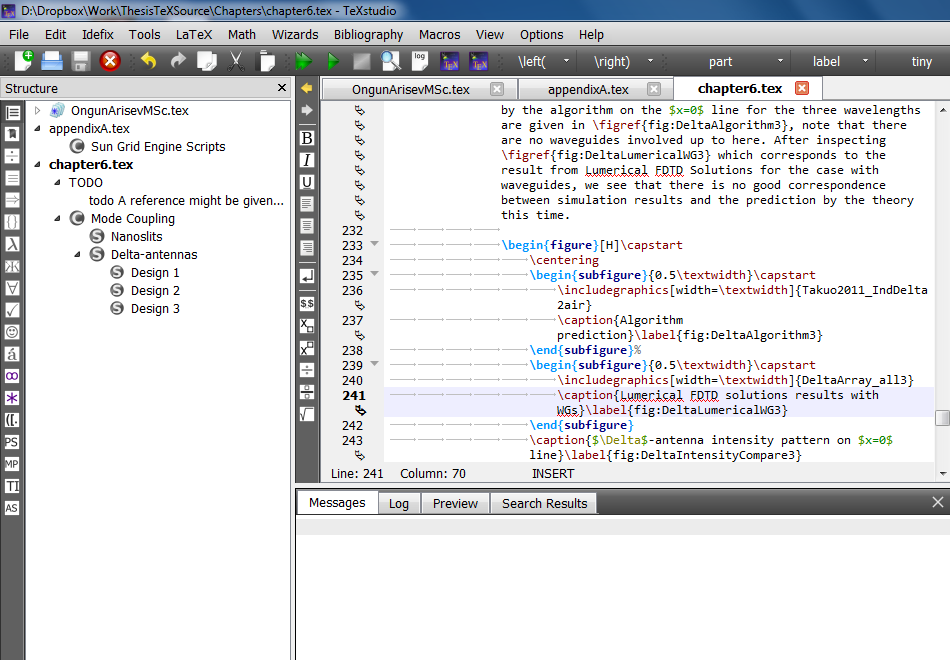
\includegraphics[width=0.99\linewidth]{res/images/latex.jpg}
			\caption{Software per la stesura dei documenti}
		\end{figure} 
		\paragraph{Draw.io} \mbox{}\\
		Draw.io è una piattaforma online per la produzione di varie tipologie di diagrammi, tra cui gli UML. \newline
		\centerline{\url{https://www.draw.io/}}
	
\subsection{Gestione della Qualità}
	\subsubsection{Scopo}
	Lo scopo è di garantire che il prodotto e i servizi offerti rispettino gli obiettivi di qualità, e che i bisogni del proponente siano soddisfatti.
	\subsubsection{Aspettative}
	Mediante la Gestione della Qualità si intende ottenere:
	\begin{itemize}
		\item qualità nell'organizzazione, nei suoi processi;
		\item qualità nel prodotto;
		\item qualità provata oggettivamente;
		\item soddisfazione finale di cliente e proponente;
	\end{itemize}
	\subsubsection{Descrizione}
	Per la trattazione approfondita della gestione della qualità si fa riferimento al Piano di Qualifica, dove sono descritte le modalità utilizzate per garantire la qualità nello sviluppo del progetto. In particolare, in tale documento:
	\begin{itemize}
		\item sono presentati gli standard utilizzati;
		\item sono individuati i processi di interesse negli standard;
		\item sono individuati gli attributi del software più significativi per il progetto.
	\end{itemize}
	Per ogni processo si mostrano:
	\begin{itemize}
		\item gli obiettivi da perseguire;
		\item le strategie da applicare;
		\item le metriche da utilizzare.
	\end{itemize}
	al fine di migliorare e controllare i processi e i loro risultati.
	Per ogni prodotto si mostrano:
	\begin{itemize}
		\item gli obiettivi da perseguire;
		\item le metriche da utilizzare;
	\end{itemize}
	al fine di ottenere software e documentazione di sufficiente qualità.
	\subsubsection{Attività}
	Le tre attività principali del processo sono:
	\begin{itemize}
		\item \textbf{Pianificazione}: porsi degli obiettivi di qualità, definire strategie per raggiungerli e disporre di conseguenza le persone e le risorse nel modo migliore;

		\item \textbf{Valutazione}: mettere in atto la pianificazione, applicando i criteri, misurando, monitorando i risultati; 
		\item \textbf{Reazione}: sulla base dei risultati, adattare le proprie strategie, criteri, piani.
	\end{itemize}
	\subsubsection{Strumenti}
	Gli strumenti predefiniti per la qualità sono: 
	\begin{itemize}
		\item forniti dallo standard \textit{ISO 12207};
		\item le metriche.
	\end{itemize} 
		
\subsection{Verifica}
	\subsubsection{Scopo}
	Il processo di verifica ha per scopo l'ottenimento di prodotti corretti, coesi e completi. Gli oggetti della verifica sono il software e i documenti. 
	\subsubsection{Aspettative}
	Il corretto svolgimento del processo di verifica rispetta i punti seguenti:	
	\begin{itemize}
		\item La verifica è effettuata seguendo procedure definite;
		\item Vi sono criteri chiari e affidabili da seguire per verificare;
		\item I prodotti passano attraverso fasi successive, ognuna delle quali è verificata;
		\item Dopo la verifica il prodotto è in uno stato stabile;
		\item la verifica rende possibile la validazione.
	\end{itemize}
	\subsubsection{Descrizione}
	Il processo di verifica prende in input ciò che è già stato prodotto, e lo restituisce in uno stato conforme alle aspettative. Per ottenere tale risultato ci si affida a processi di analisi e di test.
	\subsubsection{Attività}
		\paragraph{Analisi} \mbox{}\\
		Il processo di analisi si suddivide in analisi statica e analisi dinamica.
			\subparagraph{Analisi statica} \mbox{}\\
			L'analisi statica effettua controlli su documenti e codice, di cui valuta e applica la correttezza (intesa come assenza di errori e difetti), la conformità a regole e la coesione dei componenti.\newline Per effettuare analisi statica esistono metodi manuali di lettura (attuati da persone) e metodi formali (attuati da macchine). I metodi manuali sono due:
			\begin{itemize}
				\item \textbf{Walkthrough}: i vari componenti del team analizzano gli oggetti nella loro totalità per cercare anomalie; non si sà in partenza se ci siano difetti, quali e dove siano;
				\item \textbf{Inspection}: i verificatori usano liste di controllo per fare ispezione cercando errori specifici in parti specifiche.
			\end{itemize}
			A seguire sono descritte le liste di controllo utilizzabili per le ispezioni. Si prevede l'ampliamento delle viste al progredire delle ispezioni e degli errori trovati.
			
			


		
			\begin{table}[H]
				\centering\renewcommand{\arraystretch}{1.5}
				\arrayrulecolor{white}
				\begin{tabular}{c|c}
					
					\rowcolorhead
					{\colorhead \textbf{Oggetto}} &
					{\colorhead \textbf{Controllo} }\\
					
					\rowcolorlight
					{\colorbody Formato data} & {\colorbody Deve seguire il formato americano \textit{YYYY-MM-GG}} 
					\\
					
					\rowcolordark
					{\colorbody Sintassi} & {\colorbody  La frase è troppo complessa e può essere semplificata } 
					\\	
					
					\rowcolorlight
					{\colorbody Parte mancante} & {\colorbody Controllare titoli vuoti o sezioni di grandezza insolita} 
					\\
					
					\rowcolordark
					{\colorbody Forma dei verbi} & {\colorbody In generale è preferibile il presente indicativo} 
					\\
					
					\rowcolorlight
					{\colorbody Punteggiatura degli elenchi} & {\colorbody Ogni voce termina in \textbf{";"} eccetto l'ultima che termina in \textbf{"."}} 
					\\
				\end{tabular}
				\caption{Errori frequenti nei documenti}
			\end{table}

			% da aggiungere quando si fa codice				
														
			\subparagraph{Analisi dinamica} \mbox{}\\
			L’analisi dinamica è una tecnica di analisi del prodotto software che richiede la sua esecuzione. Viene effettuata  mediante dei test che verificano se il prodotto funziona e se ci sono anomalie. 
			
		\paragraph{Test} \mbox{}\\	
		I test sono l'attività fondamentale dell'analisi dinamica: verificano che il codice scritto funzioni correttamente.
		Per ogni test devono  essere definiti i seguenti parametri:
		\begin{itemize}
			\item \textbf{Ambiente}: sistema hardware e software sul quale verrà eseguito il test del prodotto;
			\item \textbf{Stato iniziale}: lo stato iniziale dal quale il test viene eseguito;
			\item \textbf{Input}: input inserito;
			\item \textbf{Output}: output atteso;
			\item \textbf{Istruzioni aggiuntive}: ulteriori istruzioni su come va eseguito il test e su come vanno interpretati i risultati ottenuti.
		\end{itemize}
		Test ben scritti devono:
		\begin{itemize}
			\item Essere ripetibili;
			\item Specificare l'ambiente di esecuzione;
			\item Specificare input e output richiesti;
			\item Avvertire di possibili side effect;
			\item Fornire informazioni sui risultati dell'esecuzione in forma di file di log.
		\end{itemize}	
			
		Ci sono vari tipi di test del software, ognuno dei quali ha diverso oggetto di verifica e scopo.
			\subparagraph{Test di unità} \mbox{}\\
			I test di unità si eseguono su unità di software. Questi test si concentrano sul funzionamento delle unità individuali. Dati gli input possibili in un unità, si suddividono gli input in partizioni di equivalenza e si prova se gli input attesi danno gli output attesi. Le singole unità possono essere testate con l'ausilio di driver e stub.
			\subparagraph{Test di integrazione} \mbox{}\\
			Dopo aver superato i test di unità, le unità vengono assemblate in componenti progressivamente più grandi. Il test di integrazione si concentra sulle interfacce tra i componenti. Un agglomerato che supera il test di integrazione costituisce quindi una nuova unità per un agglomerato di grandezza maggiore. Questa procedura si ripete fino a raggiungere la grandezza totale del sistema.
			\subparagraph{Test di sistema} \mbox{}\\\\
			Il sistema viene testato nella sua interezza, integrati tutti i suoi componenti. Ci si concentra sulle interazioni tra i componenti, sul comportamento emergente\glosp delle caratteristiche del sistema e sulla copertura\glosp di tutte le funzionalità. Questo test porta alla luce le ipotesi errate che i diversi sviluppatori fanno su parti del software sviluppate da altri.
			In questa fase ci si assicura che il sistema rispetti tutte le specifiche definite nell'\textit{AdR}.
			\subparagraph{Test di regressione} \mbox{}\\
			Si effettua di seguito a una modifica del sistema, e consiste nella riesecuzione dei test esistenti: si combina bene con l'automazione dei test.
			\subparagraph{Test di collaudo} \mbox{}\\
			Simile al test di sistema, ma eseguito con la collaborazione dei committenti, si occupa di verificare il prodotto intero, e in particolare la sua conformità alle richieste. Il superamento del test di collaudo garantisce che il software è pronto per essere rilasciato.
	\subsubsection{Strumenti}
		\paragraph{Verifica ortografica} \mbox{}\\
		Viene utilizzata la verifica dell'ortografia in tempo reale, strumento integrato in TexStudio che sottolinea in rosso le parole errate secondo la lingua italiana.
		\paragraph{Validazione W3C} \mbox{}\\
		Per la validazione delle pagine di markup HTML viene utilizzato lo strumento offerto dal W3C, raggiungibile al seguente indirizzo: \newline
		\centerline{\url{https://validator.w3.org/}} \newline
		Per la validazione dei fogli di stile CSS viene utilizzato lo strumento offerto dal W3C, raggiungibile al seguente indirizzo: \newline
		\centerline{\url{https://jigsaw.w3.org/css-validator/}} \newline

		%\paragraph{Metriche} ????
		% da fare
\subsection{Validazione}
	\subsubsection{Scopo}
	Lo scopo della validazione stabilire è portare il prodotto al rilascio. Dopo la validazione, è garantito che il software rispetti i requisiti e soddisfi i bisogni del committente. 
	\subsubsection{Attività}
	Per validare il prodotto si seguo i punti seguenti:
	\begin{itemize}
		\item identificare gli oggetti da validare;
		\item identificare una strategia con delle procedure di validazione: si possono riutilizzare le procedure di verifica;
		\item applicare la strategia;
		\item valutare che i risultati rispettino le aspettative;
	\end{itemize}

\subsection{Configurazione}
	\subsubsection{Scopo}
	Lo scopo della configurazione è di creare ordine tra gli oggetti software e documentali. Gli oggetti configurati si trovano in un posto preciso, hanno uno stato che li identifica, sono modificati secondo procedure e posti sotto versionamento.
	\subsection{Versionamento} \mbox{}\\
		\paragraph{Tecnologie} \mbox{}\\
		Per le parti del progetto da versionare si è scelto di usare il sistema di versionamento distribuito \textit{Git}, usando il servizio di GitHub per ospitare la repository remota.
		\paragraph{Repository} \mbox{}\\
		Il sistema di versionamento usato è \textit{Git}, noto sistema di controllo versione distribuito. I membri del team possono usare lo strumento sia da linea di comando sia attraverso software che ne migliorano l'usabilità, come GitFlow, GitKraken. La versione comune e ufficiale del progetto è  ospitata in una repository pubblica su Github all'indirizzo \url{https://github.com/8LabSolutions/Soldino}.
		\paragraph{Struttura del repository} \mbox{}\\
		Ci sono due tipi di repository:
		\begin{itemize}
			\item \textbf{locale}: ogni studente possiede una copia locale del progetto su cui lavorare;
			\item \textbf{remota}: ospitata su \textit{GitHub}, è la versione di riferimento per tutto il team e quella disponibile all'esterno;
		\end{itemize}						
		Entrambe i tipi di repository sono organizzati in cartelle:
		\begin{itemize}
			\item \textbf{latex}: qui risiedono i file di carattere generale, come i file relativi a package, che vengono inseriti in tutti i documenti, e i template, che sono usati come riferimento per nuovi documenti di struttura già definita;
			\item \textbf{guide}: qui si trovano delle brevi guide di carattere pratico, come brevi spiegazioni per applicare comandi latex poco conosciuti;
			\item \textbf{RR}: qui si trovano i documenti, suddivisi tra esterni ed interni, appartenenti alla Revisione dei Requisiti;
			\item Saranno aggiunte in futuro cartelle distinte nominate \textbf{RP}, \textbf{RQ} e \textbf{RA} contenenti i file delle rispettive consegne.
		\end{itemize}
		Lo scopo della suddivisione dei file per revisioni è di evidenziare il lavoro svolto per ogni consegna, e di rendere ben tracciabili i file che le riguardano.
		\paragraph{Tipi di file e .gitignore} \mbox{}\\
		I file di interesse per il progetto sono:
		\begin{itemize}
			\item file .tex di \LaTeX{};
			\item file .pdf che sono oggetto di consegna;
			\item alcuni file testuali e immagini di supporto ai precedenti.
		\end{itemize}			
		Il file \textit{.gitignore} presente al livello più esterno della repository elenca ed esclude tutti i file che vengono prodotti durante lo sviluppo del progetto ma non sono rilevanti per la consegna.

		\paragraph{Utilizzo di Git} \mbox{}\\
		La repository \textit{git} è composta di vari branch, per lavorare in modo modulare e collaborativo. Ogni membro del team lavora su un branch in un dato istante.\newline 
		Per lavorare su git si consiglia questa procedura:
			\begin{enumerate}
			\item scelta del \textit{branch} corretto;
			\item \textit{pull} dalla repository remota per aggiornare la propria repository locale;
			\item svolgimento del lavoro, che consiste nella modifica dei propri file locali;
			\item \textit{add} dei file al sistema di versionamento;
			\item commit dei file aggiunti, corredato di un messaggio che identifica le modifiche;
			\item push del commit nella repository remota;
		\end{enumerate}
		\paragraph{Gestione delle modifiche}
		Tutti i membri del team possono liberamente modificare i file in ogni branch, a eccezione del branch master, per il quale occorre fare una pull request e ottenere l'approvazione di un'altro membro.\newline

		Per effettuare modifiche maggiori sui contenuti o la struttura dei file si prevede di:
		\begin{itemize}
			\item contattare l'autore dell'oggetto da modificare;
			\item suggerire la modifica da effettuare;
			\item valutare insieme la modifica;
			\item se la valutazione è positiva, effettuare la modifica;
		\end{itemize}
		Per modifiche minori, come correzioni grammaticali o miglioramenti sintattici, si consiglia di modificare indipendentemente.\newline
		In ambo i casi è opportuno commentare i propri commit con chiarezza per risalire facilmente alle modifiche.
	\subsection{Attività}
	Le attività di configurazione includono:
	\begin{itemize}
		\item identificare gli oggetti di configurazione;
		\item porli sotto versionamento;
		\item apportare modifiche in modo controllato;
		\item controllare l'immagazzinamento, l'utilizzo, la consegna finale.
	\end{itemize}

